% !TeX program = xelatex
% !BIB program = biber
% !TeX spellcheck = ru_RU
\documentclass[14pt,a4paper]{extarticle}
\usepackage{fontspec}
\IfFontExistsTF{Times New Roman}
  {\setmainfont{Times New Roman}}
  {\setmainfont{Liberation Serif}}
\usepackage[a4paper,left=30mm,right=10mm,top=20mm,bottom=20mm]{geometry}
\usepackage[english,russian]{babel}
\usepackage[unicode,colorlinks,filecolor=black,citecolor=black,linkcolor=black]{hyperref}
\usepackage{booktabs}
\usepackage{amsmath} 
\usepackage{amssymb}
\usepackage{listings}
\usepackage{xcolor}
\usepackage{graphicx}
\graphicspath{ {./} }
\usepackage{enumitem}
\usepackage{siunitx}
\usepackage[font={footnotesize,it}]{caption}
\usepackage{tabularx}
\usepackage{float}
\usepackage{csquotes}
\usepackage[backend=biber,style=numeric,sorting=none]{biblatex}
\addbibresource{references.bib}
\usepackage{setspace}
\usepackage{titlesec}
\usepackage{tocloft}

\titleformat{\section}
  {\normalfont\fontsize{16}{19}\bfseries\filcenter}
  {Глава \thesection.}
  {1em}
  {}
\titleformat{name=\section,numberless}
  {\normalfont\fontsize{16}{19}\bfseries\filcenter}
  {}
  {0pt}
  {}
\titleformat{\subsection}
  {\normalfont\normalsize\bfseries\filcenter}
  {\thesubsection.}                 
  {1em}                            
  {}
\titleformat{\subsubsection}
  {\normalfont\normalsize\bfseries\filcenter}
  {\thesubsubsection.}               
  {1em}                            
  {}
\titlespacing*{\section}{0pt}{0pt}{\baselineskip}
\titlespacing*{\subsection}{0pt}{\baselineskip}{\baselineskip}
\titlespacing*{\subsubsection}{0pt}{\baselineskip}{\baselineskip}
\renewcommand{\cftsecpresnum}{Глава~}
\renewcommand{\cftsecaftersnum}{.}
\setlength{\cftsecnumwidth}{5.5em}
\setlength{\cftsubsecnumwidth}{3.2em}
\captionsetup[table]{position=top,justification=centering,singlelinecheck=true,labelsep=endash,font={small}}
\captionsetup[figure]{position=bottom,justification=centering,labelsep=endash,font={small}}

\definecolor{codegreen}{rgb}{0,0.6,0}
\definecolor{codeblue}{rgb}{0,0,0.6} 
\definecolor{codepurple}{rgb}{0.58,0,0.82} 
\definecolor{backcolour}{rgb}{0.98,0.98,0.98} 

\lstdefinestyle{json}{
    backgroundcolor=\color{backcolour},   
    commentstyle=\color{codegreen},
    stringstyle=\color{codepurple},
    numberstyle=\color{codeblue}\footnotesize,
    basicstyle=\ttfamily\footnotesize,
    breakatwhitespace=false,         
    breaklines=true,                 
    captionpos=b,                    
    keepspaces=true,                 
    showspaces=false,                
    showstringspaces=false,
    showtabs=false,                  
    tabsize=2,
    frame=single,                    
    rulecolor=\color{black}
}
\setcounter{secnumdepth}{5}
\setcounter{biburllcpenalty}{7000}
\setcounter{biburlucpenalty}{8000}
\setlength{\parindent}{1.25cm}
\setlength{\parskip}{0pt}
\begin{document}
\onehalfspacing
\pagestyle{plain}
\sloppy
\begin{titlepage}
\thispagestyle{empty}
\begin{center}
\normalsize
ФЕДЕРАЛЬНОЕ ГОСУДАРСТВЕННОЕ АВТОНОМНОЕ\\
ОБРАЗОВАТЕЛЬНОЕ УЧРЕЖДЕНИЕ\\
ВЫСШЕГО ОБРАЗОВАНИЯ\\
«НАЦИОНАЛЬНЫЙ ИССЛЕДОВАТЕЛЬСКИЙ УНИВЕРСИТЕТ\\
ВЫСШАЯ ШКОЛА ЭКОНОМИКИ»

\vspace{4mm}

\textbf{Факультет информатики, математики и компьютерных наук}

\vfill

\textit{Пестов Лев Евгеньевич}\\[4mm]

\textbf{КУРСОВАЯ РАБОТА}\\[6mm]

Разработка системы семантической сегментации дорожной сцены\\
с акцентом на сегментацию слабоконтрастных объектов\\[5mm]

\normalsize{по направлению подготовки 01.03.02 «Прикладная математика и информатика»\\
образовательная программа «Компьютерные науки и технологии»}

\end{center}

\vfill
\hfill
\begin{minipage}{0.5\textwidth}
\raggedleft{Научный руководитель\\
доцент кафедры информационных\\систем и технологий\\[2mm]
Улитин Борис Игоревич\\[5mm]
Соруководитель\\
приглашённый преподаватель\\кафедры прикладной математики\\и информатики\\[2mm]
Сенников Андрей Олегович}
\end{minipage}
\vfill
\begin{center}
Нижний Новгород, 2026г.
\end{center}
\end{titlepage}
\setcounter{page}{2}
\newpage

\renewcommand{\contentsname}{Оглавление}
\tableofcontents
\newpage

\section*{Введение}
\addcontentsline{toc}{section}{Введение}

\textbf{Актуальность темы.} Системы автономного вождения и помощи водителю (ADAS) предъявляют высокие требования к устойчивости алгоритмов компьютерного зрения. Современные методы семантической сегментации демонстрируют высокие показатели качества (mIoU > 80\%) на стандартных бенчмарках, включая Cityscapes, где изображения обычно получены при хорошем освещении и благоприятной погоде. В реальной дорожной сцене часто возникают туман, дождь, снегопад, сумерки и ночное освещение. Эти факторы снижают контрастность объектов и ухудшают качество моделей, обученных на данных с нормальной видимостью.

Наиболее критичны ошибки на слабоконтрастных объектах: пешеходах в темной одежде, велосипедистах и удаленных транспортных средствах, сливающихся с фоном. Для ADAS такие ошибки повышают риск неверной оценки дорожной обстановки. Сбор и пиксельная разметка данных для всех погодных условий требуют значительных ресурсов, поэтому в работе рассматриваются методы переноса моделей из домена нормальной видимости в домены со сложными условиями съемки без полной переразметки данных.

\textbf{Проблема исследования} заключается в существенном падении точности (Domain Shift) современных алгоритмов семантической сегментации при переходе от домена с хорошей видимостью к домену с неблагоприятными погодными условиями, особенно в части распознавания малых и слабоконтрастных объектов.

\textbf{Цель работы} состоит в разработке и исследовании методики повышения качества семантической сегментации дорожных сцен в сложных погодных условиях (туман, ночь, дождь) с использованием методов доменной адаптации и модификации процесса обучения.

Для достижения поставленной цели необходимо решить следующие \textbf{задачи}:
\begin{enumerate}
    \item Провести обзор современных архитектур нейронных сетей (CNN и Transformer-based) для задачи семантической сегментации.
    \item Изучить проблему доменного сдвига (Domain Shift) и методы повышения обобщающей способности моделей (Data Augmentation, Domain Adaptation).
    \item Реализовать базовый пайплайн обучения (baseline) на наборе данных Cityscapes и оценить его качество на данных со сложными погодными условиями (ACDC).
    \item Разработать и внедрить модификации (аугментации, функции потерь), направленные на улучшение распознавания слабоконтрастных объектов.
    \item Провести сравнительный анализ результатов и оценить качество предложенных модификаций.
\end{enumerate}

\textbf{Объект исследования:} алгоритмы семантической сегментации изображений дорожных сцен.

\textbf{Предмет исследования:} методы повышения устойчивости нейронных сетей к изменению визуальных условий (освещение, погода) и снижению контраста.

\textbf{Методы исследования.} В работе применяются анализ и систематизация литературы по семантической сегментации и доменной адаптации, а также сравнительный вычислительный эксперимент с единым протоколом оценки. Каждая конфигурация обучается на одних и тех же данных и проверяется на ACDC validation. Качество измеряется метриками mIoU и Pixel Accuracy в разбивке по четырём погодным условиям. Анализ ошибок проводится на уровне отдельных классов и дополняется визуальными примерами предсказаний.

\textbf{Научная новизна} работы состоит в сравнении четырёх архитектурных подходов --- классической CNN, современного CNN-бэкбона с деформируемыми свёртками, трансформера для сегментации и foundation-модели с self-supervised предобучением --- в рамках единого протокола оценки переноса Cityscapes→ACDC без использования целевых данных при обучении. В той же постановке последовательно проверен вклад source-only модификаций (фотометрические аугментации, частотный перенос стиля, consistency-регуляризация) и двух вариантов UDA-lite: offline self-training на pseudo-labels и online EMA-teacher с ClassMix.

\textbf{Теоретическая значимость} результатов состоит в количественном разграничении вклада архитектуры и вклада стратегии обучения в качество переноса. В частности, показано, что разрыв между крайними архитектурами в source-only постановке превышает суммарный прирост от всех рассмотренных модификаций обучения, что указывает на доминирующую роль бэкбона при ограниченном доступе к целевому домену.

\textbf{Практическая ценность.} Конфигурация DINOv2-Small~E3 пригодна для применения в задачах сегментации при неблагоприятных условиях съёмки без какого-либо доступа к целевому домену. Если неразмеченные изображения целевого домена доступны, DINOv2-Small~U2 обеспечивает наилучшее итоговое качество из всех проверенных вариантов. Оба сценария не требуют пиксельной разметки target-данных, что существенно снижает стоимость адаптации модели к новым условиям съёмки.

\newpage

\section{Теоретические основы семантической сегментации и доменной устойчивости}

\subsection{Семантическая сегментация дорожной сцены}

\subsubsection{Формализация задачи pixel-wise классификации}
Семантическая сегментация представляет собой задачу плотной (pixel-wise) классификации, в которой каждому пикселю входного изображения сопоставляется метка класса из заранее заданного множества. Формально, пусть задано входное изображение $X \in \mathbb{R}^{H \times W \times C}$, где $H$ и $W$ --- пространственные размеры изображения (высота и ширина), а $C$ --- количество каналов (обычно $C=3$ для RGB-изображений). Пусть $\mathcal{K} = \{1, 2, \dots, K\}$ --- множество целевых семантических классов, характерных для дорожной сцены (например, дорога, тротуар, здания, транспорт, пешеходы и т.д.).

Цель модели семантической сегментации (нейронной сети), параметризованной весами $\theta$, заключается в поиске отображения $f_\theta$:
\begin{equation}
    f_\theta : \mathbb{R}^{H \times W \times C} \to \mathbb{R}^{H \times W \times K},
\end{equation}
которое преобразует входное изображение в тензор логитов $Z \in \mathbb{R}^{H \times W \times K}$. Для каждого пространственного положения (пикселя) с координатами $(i, j)$ сеть предсказывает вектор $z_{i,j} \in \mathbb{R}^K$.

Вероятностное распределение принадлежности пикселя к каждому из $K$ классов получается путем применения функции \textit{softmax} вдоль канала классов:
\begin{equation}
    p_{i,j}^{(k)} = \frac{\exp\left(z_{i,j}^{(k)}\right)}{\sum_{c=1}^K \exp\left(z_{i,j}^{(c)}\right)},
\end{equation}
где $p_{i,j}^{(k)}$ --- предсказанная вероятность того, что пиксель $(i, j)$ принадлежит классу $k$.

Итоговая предсказанная маска сегментации $\hat{Y} \in \mathcal{K}^{H \times W}$ формируется путем выбора класса с максимальной вероятностью для каждого пикселя:
\begin{equation}
    \hat{y}_{i,j} = \arg\max_{k \in \mathcal{K}} p_{i,j}^{(k)}.
\end{equation}

В процессе обучения модели наиболее распространенным функционалом потерь является средняя категориальная кросс-энтропия (Categorical Cross-Entropy, CCE). Если $y_{i,j}$ --- истинная метка класса для пикселя $(i, j)$, представленная в виде one-hot вектора (где $y_{i,j}^{(k)} = 1$, если пиксель принадлежит классу $k$, и $0$ иначе), то функция потерь имеет вид:
\begin{equation}
    \mathcal{L}_{CE} = - \frac{1}{H \cdot W} \sum_{i=1}^{H} \sum_{j=1}^{W} \sum_{k=1}^{K} y_{i,j}^{(k)} \log\left(p_{i,j}^{(k)}\right).
\end{equation}

В отличие от классификации изображений и детектирования объектов, сегментация требует одновременно семантической точности и точной локализации границ. В задачах автономного вождения модель должна выделять крупные структуры дорожной сцены и малые слабоконтрастные объекты, включая удаленных пешеходов и дорожные знаки. Поэтому качество сегментации чувствительно к доменному сдвигу (domain shift) между распределением обучающих данных (source domain) и распределением данных в целевом сценарии (target domain), например при изменении погоды или времени суток.

\subsubsection{Основные метрики: mIoU, class-wise IoU, Pixel Accuracy}
Для количественной оценки качества моделей семантической сегментации используются метрики, основанные на вычислении площадей перекрытия предсказанных и истинных масок. В основе вычислений лежат базовые элементы матрицы ошибок (Confusion Matrix), рассчитываемые независимо для каждого класса $k$:
\begin{itemize}
    \item $TP_k$ (True Positives) --- количество истинно-положительных пикселей (пиксели, верно отнесенные к классу $k$);
    \item $FP_k$ (False Positives) --- количество ложно-положительных пикселей (пиксели, ошибочно отнесенные к классу $k$);
    \item $FN_k$ (False Negatives) --- количество ложно-отрицательных пикселей (пиксели класса $k$, отнесенные моделью к другому классу);
    \item $TN_k$ (True Negatives) --- количество истинно-отрицательных пикселей (пиксели других классов, корректно не отнесенные к классу $k$).
\end{itemize}

Основная метрика качества в работе --- \textbf{mIoU} (mean Intersection over Union, среднее пересечение над объединением). Сначала вычисляется \textbf{class-wise IoU} для каждого класса $k$: отношение площади пересечения предсказанной маски и ground truth маски к площади их объединения:
\begin{equation}
    \text{IoU}_k = \frac{TP_k}{TP_k + FP_k + FN_k}.
\end{equation}

Значение $\text{IoU}_k$ лежит в диапазоне от $0$ до $1$. Анализ class-wise IoU показывает, на каких классах модель ошибается чаще всего. В дорожных сценах к таким классам часто относятся \textit{bicycle}, \textit{fence} и \textit{pole}: они занимают малую площадь и имеют сложную геометрию \cite{cordts2016cityscapes}.

Интегральная метрика mIoU рассчитывается как арифметическое среднее значений IoU по всем $K$ классам:
\begin{equation}
    \text{mIoU} = \frac{1}{K} \sum_{k=1}^{K} \text{IoU}_k.
\end{equation}
В отличие от простой пиксельной точности, mIoU устойчивее к сильному дисбалансу классов, типичному для дорожных сцен \cite{cordts2016cityscapes}: класс «дорога» может занимать значительную часть изображения, а класс «светофор» --- менее долей процента.

Дополнительно в работе используется базовая метрика \textbf{Pixel Accuracy (PA)} --- доля корректно классифицированных пикселей по отношению к общему числу пикселей изображения:
\begin{equation}
    \text{PA} = \frac{\sum_{k=1}^{K} TP_k}{\sum_{k=1}^{K} (TP_k + FP_k + FN_k + TN_k)} = \frac{\sum_{i=1}^{H} \sum_{j=1}^{W} \mathbb{I}(\hat{y}_{i,j} = y_{i,j})}{H \cdot W},
\end{equation}
где $\mathbb{I}(\cdot)$ --- индикаторная функция, равная $1$ при выполнении условия и $0$ в противном случае. Хотя PA легко интерпретируется, она может быть обманчиво высокой при доминировании фоновых классов, поэтому используется лишь в качестве вспомогательного индикатора.

Для оценки устойчивости моделей в \textit{adverse}-условиях метрики отдельно агрегируются по подмножествам целевого датасета: \textit{fog}, \textit{night}, \textit{rain}, \textit{snow} в ACDC. Такое разбиение показывает, при каких погодных и оптических искажениях качество сегментации снижается сильнее.

\subsection{Архитектурные подходы}

\subsubsection{CNN-подходы (DeepLabV3+ как классический baseline)}
Сверточные архитектуры долгое время оставались основным классом моделей для семантической сегментации. В работе в качестве классического подхода рассматривается \textbf{DeepLabV3+ \cite{chen2018deeplabv3plus}}, сочетающая энкодер-декодерную схему, модуль \textit{Atrous Spatial Pyramid Pooling} и \textit{dilated} свертки для расширения эффективного рецептивного поля без потери разрешения признаков. Такая архитектура учитывает контекст на нескольких масштабах и уточняет границы объектов, что важно для дорожных сцен с тонкими структурами и малыми объектами. В оригинальной статье авторы сообщают о результате \textbf{82.1\% mIoU} на тестовом наборе \textit{Cityscapes} и \textbf{89.0\% mIoU} на \textit{PASCAL VOC 2012} без дополнительного post-processing. Здесь DeepLabV3+ используется как CNN-baseline для сравнения с трансформерными и foundation-подходами.

\subsubsection{Transformer-подходы (SegFormer)}
\textbf{SegFormer \cite{xie2021segformer} }относится к эффективным трансформерным архитектурам для семантической сегментации. Модель использует иерархический энкодер, который формирует признаки на нескольких масштабах без позиционного кодирования, и легкий MLP-декодер. Декодер объединяет разномасштабные признаки для построения итоговой маски, сохраняя баланс между качеством сегментации и вычислительной сложностью. В оригинальной статье конфигурация \textit{SegFormer-B5} достигает \textbf{84.0\% mIoU} на тестовом наборе \textit{Cityscapes}, а вариант \textit{SegFormer-B4} показывает \textbf{51.8\% mIoU} на \textit{ADE20K}. В работе используется конфигурация \textit{SegFormer-B2}, реализованная через библиотеку \texttt{segmentation\_models\_pytorch}; она выступает сильным трансформерным baseline и не относится к foundation-моделям в строгом смысле.

\subsubsection{CNN-based foundation backbones (InternImage)}
\textbf{InternImage \cite{wang2023internimage} }представляет собой CNN-based foundation-модель, в которой в качестве основного оператора используется \textit{DCNv3} --- деформируемая свертка с большим эффективным рецептивным полем и адаптивным пространственным агрегированием признаков. Архитектура строится как иерархический четырехстадийный бэкбон, а ее блоки сочетают свойства современных CNN и transformer-подобный дизайн, включая \textit{Layer Normalization}, \textit{feed-forward network} и \textit{GELU}. Поэтому InternImage рассматривается как промежуточный вариант между классическими сверточными сетями и крупными vision foundation models.

\subsubsection{\textit{Foundation}-бэкбоны в сегментации (DINOv2)}
Foundation-подходы используют предварительное обучение на масштабных и разнообразных наборах изображений без разметки \textit{(self-supervised learning)}, что существенно повышает переносимость признаков между различными доменами и задачами. \textbf{DINOv2 \cite{oquab2023dinov2}} --- современная архитектура на базе \textit{Vision Transformer}, которая благодаря обучению с дистилляцией и специальным целевым функциям формирует богатые универсальные визуальные представления. В оригинальной статье показано, что даже замороженный бэкбон DINOv2 в связке с \textit{ViT-Adapter} достигает \textbf{60.2\% mIoU} на \textit{ADE20K}, \textbf{86.9\% mIoU} на \textit{Cityscapes} и \textbf{89.0\% mIoU} на \textit{Pascal VOC}.

\textbf{DINOv2-Small} используется для проверки гипотезы о том, что предобученные универсальные признаки повышают устойчивость сегментации при низкой видимости, низком контрасте и сложной погоде. Для плотного предсказания поверх замороженного или дообучаемого (fine-tuning) бэкбона DINOv2 применяется легковесный линейный декодер (\texttt{LinearDecoder}). Он преобразует последовательность патч-токенов в двумерное пространственное представление и восстанавливает признаки до исходного разрешения изображения с помощью билинейной интерполяции.

\subsection{Domain Shift: DG, UDA, FDA --- термины и различия}

При сегментации дорожных сцен качество модели на обучающем распределении и в новом визуальном домене может существенно различаться. Исходный домен в работе --- Cityscapes \cite{cordts2016cityscapes}: городские сцены при сравнительно благоприятной видимости. Целевой домен --- ACDC \cite{sakaridis2021acdc}: туман, ночь, дождь и снег. Доменный сдвиг формально записывается как
\begin{equation}
    P_s(X, Y) \neq P_t(X, Y),
\end{equation}
где $P_s$ и $P_t$ --- распределения исходного и целевого доменов, $X$ --- изображение, $Y$ --- карта меток. В попиксельной задаче сдвиг затрагивает цвет, контраст, видимость границ, различимость мелких классов и частоту ошибок на тонких структурах.

\begin{figure}[H]
    \centering
    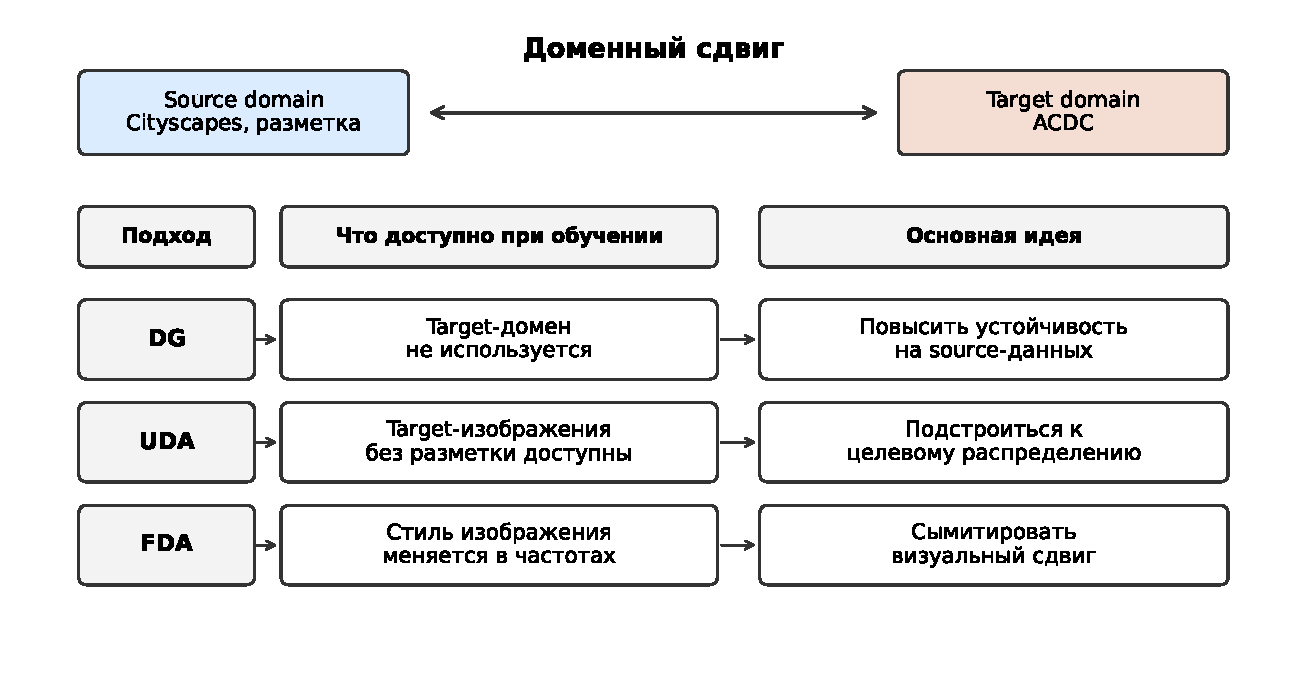
\includegraphics[width=0.92\textwidth]{domain_shift_scheme.pdf}
    \caption{Различие между DG, UDA и FDA с точки зрения доступа к целевому домену и основной идеи метода.}
    \label{fig:domain_shift_scheme}
\end{figure}

\subsubsection{DG (Domain Generalization): обучение без target-домена}

\textbf{Domain Generalization (DG)} обучает модель на одном или нескольких исходных доменах без какого-либо доступа к target-данным. Цель --- не подстройка под конкретный набор, а признаки, которые слабо зависят от условий съемки. Такая постановка анализируется в обзоре \cite{zhou2022domain}.

Эксперименты \textbf{E0--E4} соответствуют source-only / DG-style постановке: разметка берется только из Cityscapes, а ACDC используется для проверки переноса. Weather-аугментации и частотные преобразования применяются к source-изображениям и не задействуют ACDC при обучении.

\subsubsection{UDA (Unsupervised Domain Adaptation): обучение с неразмеченным target}

\textbf{Unsupervised Domain Adaptation (UDA)} в отличие от DG получает на этапе обучения неразмеченные изображения целевого домена. Разметка $Y_t$ недоступна, но $X_t$ хватает, чтобы оценивать target-статистику и подстраивать модель. Классическим инструментом было adversarial-выравнивание признаков \cite{ganin2016domain}; современные подходы для сегментации опираются на \textit{self-training}, \textit{pseudo-labels} и стабилизирующие приемы.

Базовая схема pseudo-label self-training отбирает только уверенные пиксели:
\begin{equation}
    \hat{y}_{t}^{(i,j)} = \arg\max_k p_{t}^{(i,j,k)}, \qquad
    \max_k p_{t}^{(i,j,k)} \geq \tau,
\end{equation}
где $\tau$ --- порог уверенности. Такой механизм не заменяет ручную разметку, но вводит в обучение информацию о структуре target-распределения. Дополнительные эксперименты \textbf{U1} и \textbf{U2} используют ACDC train без ground truth: через pseudo-labels и online teacher.

\subsubsection{FDA (Fourier Domain Adaptation): частотная техника адаптации}

\textbf{Fourier Domain Adaptation (FDA)} \cite{yang2020fda} переносит стиль между доменами в частотной области. Низкочастотная часть амплитудного спектра отвечает за внешний вид сцены: освещение, цветовую температуру, контраст, погодный оттенок. Фаза фиксирует геометрию и положение объектов \cite{yang2020fda}.

Преобразование Фурье представимо в виде
\begin{equation}
    \mathcal{F}(x) = A_x \cdot e^{i\Phi_x},
\end{equation}
а FDA подменяет амплитуду source-изображения $A_s$ амплитудой target-изображения $A_t$ в низкочастотной области \cite{yang2020fda}:
\begin{equation}
    \tilde{A}_s = (1 - M) \odot A_s + M \odot A_t,
\end{equation}
где $M$ --- маска выбранной полосы спектра. После обратного преобразования получается изображение с source-разметкой и target-внешностью. В эксперименте \textbf{E3} используется не классический FDA с ACDC, а source-only вариант: частотная модификация разнообразит стиль Cityscapes и сохраняет DG-постановку.

\subsubsection{Основной сценарий: source-only / DG-style}

Основная экспериментальная линия E0--E4 направлена на оценку переноса \textit{без} участия ACDC в обучении. Модели обучаются только на разметке Cityscapes, а ACDC используется как внешняя проверка устойчивости к погоде и низкой видимости.

\begin{table}[H]
    \centering
    \caption{Различие постановок, используемых в работе}
    \label{tab:domain_shift_modes}
    \begin{tabularx}{\textwidth}{p{2.6cm}X X}
        \toprule
        Постановка & Что доступно при обучении & Как используется в работе \\
        \midrule
        Source-only / DG-style & Размеченный Cityscapes; ACDC не используется & Основная линия E0--E4 и сравнение архитектур на ACDC validation \\
        UDA-lite & Размеченный Cityscapes и неразмеченный ACDC train & Дополнительные эксперименты U1 и U2 для DINOv2-Small \\
        FDA-style & Source-изображения с частотными преобразованиями стиля & Этап E3 как способ повышения устойчивости без target-разметки \\
        \bottomrule
    \end{tabularx}
\end{table}

Такая постановка соответствует практическому сценарию, когда размеченный датасет в благоприятных условиях доступен, а пиксельной разметки для нового погодного сценария нет. Основная серия экспериментов оценивает перенос Cityscapes $\rightarrow$ ACDC без target-данных при обучении. \textbf{UDA-lite} рассматривается отдельно, поскольку этот режим использует неразмеченные target-изображения.

\subsection{Обзор литературы и SOTA-контекст}

\subsubsection{Лидерборд \texorpdfstring{Cityscapes$\rightarrow$ACDC}{Cityscapes->ACDC}: что показывают UDA-методы}

Публичный лидерборд HyperAI \textit{Domain Adaptation on Cityscapes to ACDC} фиксирует эту постановку как отдельный mIoU-бенчмарк \cite{hyperai_cityscapes_acdc}. Несколько характерных позиций сведены в таблицу \ref{tab:hyperai_cityscapes_acdc_examples}.

\begin{table}[H]
    \centering
    \caption{Примеры результатов Cityscapes $\rightarrow$ ACDC по данным HyperAI}
    \label{tab:hyperai_cityscapes_acdc_examples}
    \begin{tabularx}{\textwidth}{p{4cm}p{2.4cm}X}
        \toprule
        Метод & mIoU, \% & Тип идеи \\
        \midrule
        SoRA & 78.8 & современная верхняя граница таблицы \\
        Rein & 77.6 & foundation-модель / domain generalization \\
        CoDA & 72.6 & chain-of-domain adaptation \\
        MIC & 70.4 & masked consistency \\
        HRDA & 68.0 & high-resolution UDA \\
        DAFormer & 55.4 & transformer-based UDA \\
        FDA (DeepLabV2) & 45.7 & частотная адаптация \\
        \bottomrule
    \end{tabularx}
\end{table}

Методы из верхней части таблицы используют сильные backbone, pseudo-labeling, teacher-student обучение, consistency-регуляризацию и обработку изображений в высоком разрешении. Характерные примеры включают DAFormer с transformer-based архитектурой и стабилизацией self-training \cite{hoyer2022daformer}, HRDA с multi-resolution обучением \cite{hoyer2022hrda} и MIC с masked consistency для target-изображений \cite{hoyer2023mic}. Во всех этих подходах при обучении доступны неразмеченные изображения ACDC. Основная серия экспериментов в работе не использует target-данные, чтобы отдельно оценить устойчивость моделей и source-only приемов.

\subsubsection{Какие идеи можно перенести в DG-постановку}

Из UDA-литературы используются отдельные приемы, совместимые с отсутствием target-разметки. \textbf{E2} проверяет class-balanced веса и focal-компонент на трудных классах. \textbf{E3} применяет частотные преобразования как FDA-style способ разнообразить стиль source-домена. \textbf{E4} добавляет consistency-регуляризацию только в source. Pseudo-labeling вынесен в \textbf{U1--U2}, поскольку он требует неразмеченного ACDC и выходит за пределы source-only постановки.

\subsubsection{Ограничения сопоставления DG-результатов с UDA-рейтинговыми результатами}

Прямое сравнение с UDA-лидербордом ограничено разным уровнем доступа к данным: лидерборд использует target-изображения в обучении, а E0--E4 используют ACDC только для оценки. Поэтому source-only этапы интерпретируются отдельно, а U1--U2 рассматриваются как UDA-lite расширение основной серии.

\newpage

\section{Данные, постановка переноса и схема экспериментов}

\subsection{Наборы данных и домены исследования}

\subsubsection{Cityscapes как исходный домен}

Исходный домен --- Cityscapes~\cite{cordts2016cityscapes}, базовый набор для сегментации городских сцен. Модель обучается на его размеченных кадрах в благоприятных условиях и проверяется на более сложном target-домене. Такая схема задает строгую проверку переноса: source-domain покрывает дневную съемку без осадков, а оценка проводится на изображениях с другим освещением и погодой.

\subsubsection{ACDC как целевой домен: fog, night, rain, snow}

Целевой домен --- ACDC~\cite{sakaridis2021acdc}, четыре неблагоприятных условия: \textit{fog}, \textit{night}, \textit{rain}, \textit{snow}. Разбиение по условиям дает возможность анализировать ошибку по типам сдвига, а не только по одному усредненному числу.

На рис.~\ref{fig:datasets_domain_examples} приведены примеры из обоих наборов. Различия между доменами затрагивают яркость, текстуры, насыщенность, видимость дальних объектов и надежность границ между классами.

\begin{figure}[H]
    \centering
    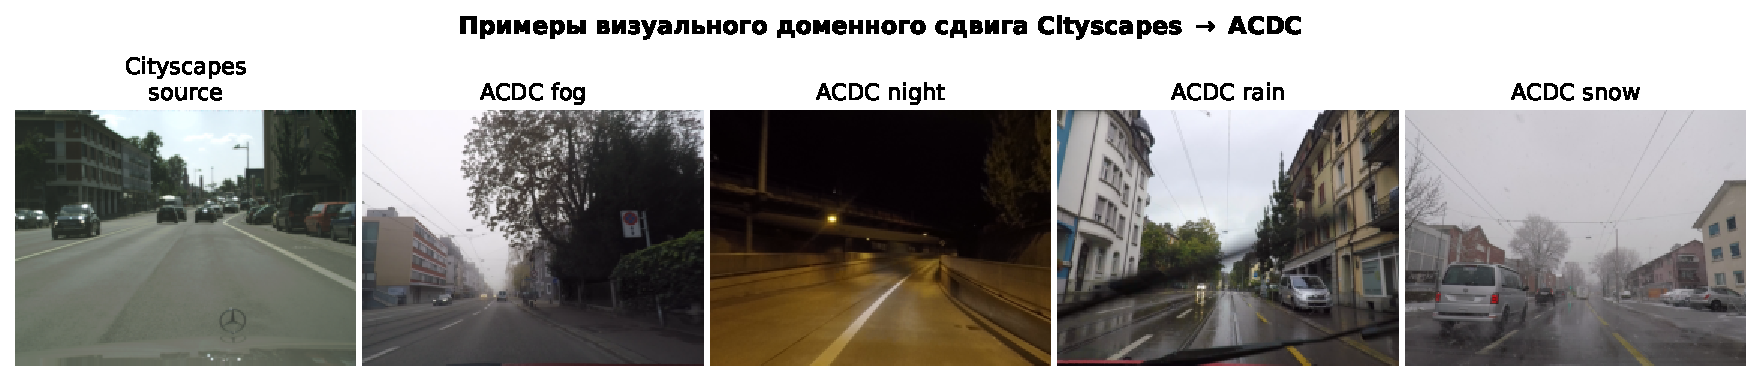
\includegraphics[width=\textwidth]{datasets_domain_examples.pdf}
    \caption{Примеры визуального сдвига между Cityscapes и погодными условиями ACDC}
    \label{fig:datasets_domain_examples}
\end{figure}

\subsubsection{Классы сегментации, разметка и подготовка данных}

Оба набора приводятся к стандартной 19-классовой схеме Cityscapes. На вход идут RGB-изображения и маски в формате \textit{trainId}; void-области ($255$) исключены из функции потерь и из расчета IoU.

Препроцессинг включает приведение к единому формату, согласованные геометрические преобразования изображения и маски и нормализацию под выбранную архитектуру. В основной линии E0--E4 ACDC выступает только тестовым доменом, его неразмеченные изображения подключаются исключительно в U1--U2.

\subsection{Метрики и критерии сравнения}

\subsubsection{Overall mIoU и Pixel Accuracy}

Основной числовой критерий --- overall mIoU на ACDC validation. По нему сравниваются архитектуры в E0 и динамика этапов E1--E4, U1 и U2. Усреднение по классам снижает влияние дисбаланса: дорога и небо занимают на порядок больше пикселей, чем светофор или знак, поэтому одна пиксельная точность слабо характеризует качество переноса.

Усреднение ведется по $K = 19$ обучаемым классам:
\begin{equation}
    \text{mIoU}_{\text{overall}} =
    \frac{1}{K}\sum_{k=1}^{K}\text{IoU}_k.
\end{equation}

Pixel Accuracy используется как вспомогательная метрика. Она показывает долю верно классифицированных пикселей и фиксирует грубую деградацию модели, но высокая PA может скрывать ошибки на малых и слабоконтрастных классах.

\begin{equation}
    \text{PA} =
    \frac{1}{|\Omega|}\sum_{(i,j)\in\Omega}
    \mathbb{I}\left(\hat{y}_{i,j}=y_{i,j}\right),
\end{equation}
где $\Omega$ --- множество валидных пикселей без игнорируемой разметки.

\subsubsection{Per-condition mIoU для fog, night, rain и snow}

ACDC валидация разбита по четырем условиям, поэтому для каждой модели отдельно считается per-condition mIoU. Усреднение по всему ACDC скрывает, на каком сдвиге случился прирост: улучшение overall mIoU может опираться целиком на туман и снег при сохранении провала ночью.

Для условия $c \in \{\textit{fog}, \textit{night}, \textit{rain}, \textit{snow}\}$ метрика считается на соответствующем подмножестве $D_c$:
\begin{equation}
    \text{mIoU}_{c} =
    \frac{1}{K}\sum_{k=1}^{K}\text{IoU}_k(D_c).
\end{equation}

\subsubsection{Class-wise IoU и качественные примеры}

Class-wise IoU используется для диагностики классов, дающих основной вклад в ошибку. Крупные области обычно сегментируются стабильнее, а тонкие и редкие классы сильнее страдают от доменного сдвига, поэтому группа слабоконтрастных и малых объектов анализируется отдельно.

\begin{equation}
    \text{IoU}_k =
    \frac{TP_k}{TP_k + FP_k + FN_k}.
\end{equation}

Качественные примеры служат дополнением к метрикам. Визуализации показывают типы ошибок: пропуск объекта, смешение близких классов, разрыв тонких структур, потерю границ в тумане, ночью, под дождем и снегом.

\newpage

\section{Реализация экспериментального пайплайна}

Все эксперименты оформлены как набор Jupyter-ноутбуков, разнесенных по назначению: обучение, генерация pseudo-labels, отдельная оценка на ACDC.

\subsection{Технический стек и организация запусков}

Основной стек: \textbf{PyTorch} для моделей и функций потерь, \textbf{PyTorch Lightning} для тренировочного цикла, \textbf{Albumentations} для синхронных преобразований изображения и маски, \textbf{TorchMetrics} для расчета IoU, \textbf{ClearML} для логирования гиперпараметров, графиков и ссылок на checkpoints.

Экспериментальный пайплайн состоит из трех этапов. Модель обучается на Cityscapes в одном из сценариев E0--E4. Затем выбранный checkpoint загружается в evaluation-ноутбук и оценивается на ACDC validation. Для UDA-lite добавляется промежуточный этап: pseudo-labels для ACDC train либо предвычисляются в U1, либо генерируются онлайн внутри цикла обучения в U2.

\subsubsection{Обучение, логирование и выбор checkpoint}

Каждый train-ноутбук фиксирует конфигурацию запуска: архитектуру, размер входа, число классов, optimizer, learning rate, batch size, состав аугментаций и путь сохранения весов. В процессе логируются train/val loss, mIoU и служебные параметры. За счет этого этапы E0--E4 сравниваются по сохраненным параметрам запусков.

Checkpoint отбирается по validation mIoU на валидационной части обучающего сценария. После выбора весов модель загружается в отдельный evaluation-ноутбук, а таблицы формируются по результатам единого контура оценки на ACDC.

\subsubsection{Аугментации и подготовка батчей}

Батч строится вокруг пары «RGB-изображение --- маска». Геометрические преобразования применяются синхронно, фотометрические --- только к изображению, чтобы не нарушать соответствие пикселей и классов. На выходе маска остается в \textit{trainId}, изображение нормализуется и переводится в тензор.

Базовый набор --- стандартный resize/crop и нормализация. Этапы E1--E3 добавляют изменения контраста, яркости, погодного стиля и частотную модификацию амплитудного спектра. E4 устроен иначе: для одного source-примера формируются weak/strong-представления, между предсказаниями вводится consistency-регуляризация.

\subsection{Архитектуры моделей}

В работе сравниваются четыре группы моделей разной сложности: классический CNN, современный convolutional backbone, transformer-based baseline и foundation-бэкбон. Эти модели задают уровни качества для последующих экспериментов.

\subsubsection{DeepLabV3+ и InternImage-Tiny как базовые ориентиры}

DeepLabV3+~\cite{chen2018deeplabv3plus} играет роль CNN-baseline. Он показывает, насколько проседает перенос Cityscapes $\rightarrow$ ACDC у классической сегментационной архитектуры без специальных механизмов устойчивости.

InternImage-Tiny~\cite{wang2023internimage} используется как современная convolutional архитектура с DCNv3-блоками. Сравнение с ним показывает вклад более выразительного backbone относительно вкладов DG/UDA-приемов.

\subsubsection{SegFormer-B2}

SegFormer-B2~\cite{xie2021segformer} используется как основной transformer-based baseline. Он проходит те же этапы E0--E4, что и DINOv2-Small; поэтому на нем проверяется, сохраняются ли эффекты аугментаций, class-balanced loss и frequency-style преобразований для другой архитектуры.

SegFormer-B2 задает уровень качества стандартной сегментационной модели при тех же данных и близком тренировочном цикле. Такое сравнение помогает отделить вклад foundation-признаков DINOv2 от вклада изменений в обучении.

\subsubsection{DINOv2-Small}

DINOv2-Small~\cite{oquab2023dinov2} --- основная модель исследования. В реализации backbone подгружается как предобученный, поверх него обучается легковесный декодер на 19 классов Cityscapes. Такая связка проверяет, насколько универсальные self-supervised признаки помогают переносу на ACDC без target-разметки.

Полная серия запусков E0--E4 и UDA-lite расширения U1--U2 выполнена для DINOv2-Small. Основанием для выбора стал результат E0: DINOv2 оказался наиболее сильной исходной архитектурой, поэтому последующие модификации пайплайна проверялись прежде всего на нем.

\newpage

\section{Результаты source-only экспериментов}

\subsection{Сравнение архитектур в E0}

\subsubsection{Общая таблица метрик на ACDC}

\begin{table}[H]
    \centering
    \caption{Baseline E0: перенос Cityscapes $\rightarrow$ ACDC validation}
    \label{tab:e0_architecture_comparison}
    \small
    \begin{tabular}{lrrrrrr}
        \toprule
        Модель & mIoU & PA & Fog & Night & Rain & Snow \\
        \midrule
        DeepLabV3+ & 0.3015 & 0.7204 & 0.4422 & 0.1363 & 0.3293 & 0.3215 \\
        InternImage-Tiny & 0.3899 & 0.7735 & 0.5380 & 0.2137 & 0.4308 & 0.3997 \\
        SegFormer-B2 & 0.4463 & 0.7685 & 0.5820 & 0.2461 & 0.4722 & 0.4553 \\
        DINOv2-Small & \textbf{0.5436} & \textbf{0.8575} & \textbf{0.6882} & \textbf{0.3350} & \textbf{0.5263} & \textbf{0.5816} \\
        \bottomrule
    \end{tabular}
\end{table}

Разброс между архитектурами в E0 заметный. DeepLabV3+ и InternImage-Tiny показывают худшие значения по каждому условию. SegFormer-B2 превосходит классические baseline. Наибольшее качество в этом сравнении показывает DINOv2-Small: overall mIoU выше SegFormer-B2 на $0.0973$, на ночи разрыв ещё заметнее ($0.3350$ против $0.2461$).

\subsubsection{Выбор моделей для основной серии}

Этапы E1--E4 проводятся для двух моделей: DINOv2-Small и SegFormer-B2. DINOv2-Small выбран как лучшая модель E0. SegFormer-B2 используется как контрольная transformer-архитектура, чтобы проверить, связаны ли эффекты E1--E4 только с foundation-бэкбоном.

\subsection{Динамика E0--E4 для DINOv2-Small}

\subsubsection{Overall и per-condition динамика}

\begin{table}[H]
    \centering
    \caption{DINOv2-Small: source-only этапы E0--E4 на ACDC validation}
    \label{tab:dinov2_e0_e4_metrics}
    \small
    \begin{tabular}{lrrrrrr}
        \toprule
        Этап & mIoU & PA & Fog & Night & Rain & Snow \\
        \midrule
        E0 & 0.5436 & 0.8575 & 0.6882 & 0.3350 & 0.5263 & 0.5816 \\
        E1 & 0.5620 & 0.8690 & 0.6940 & 0.3506 & 0.5540 & 0.5963 \\
        E2 & 0.5609 & 0.8642 & 0.6810 & 0.3510 & 0.5507 & 0.5977 \\
        E3 & \textbf{0.5711} & \textbf{0.8826} & \textbf{0.6977} & \textbf{0.3823} & 0.5542 & \textbf{0.6004} \\
        E4 & 0.5622 & 0.8727 & 0.6879 & 0.3605 & \textbf{0.5635} & 0.5836 \\
        \bottomrule
    \end{tabular}
\end{table}

Лучший source-only этап для DINOv2-Small --- \textbf{E3}: overall mIoU вырастает с $0.5436$ до $0.5711$. Самый крупный прирост по поддомену приходится на \textit{night}: $0.3350 \to 0.3823$, $+0.047$. Такой результат согласуется с целью работы, поскольку ночные сцены особенно чувствительны к низкому контрасту и ухудшению видимости.

\subsubsection{Лучший этап и откат на E4}

E1 обеспечивает устойчивый прирост над E0 за счёт фотометрических аугментаций. E2 почти не меняет overall mIoU: class-balanced loss с focal-весами улучшает часть редких классов, но одновременно снижает качество на крупных классах. E3 добавляет частотные преобразования и дает лучший source-only результат. На E4 mIoU снижается до $0.5622$. Возможное объяснение связано с тем, что consistency-регуляризация применяется только в source-домене: предсказания становятся более согласованными между weak/strong-видами одного изображения, но не приближаются к target-распределению.

\begin{figure}[H]
    \centering
    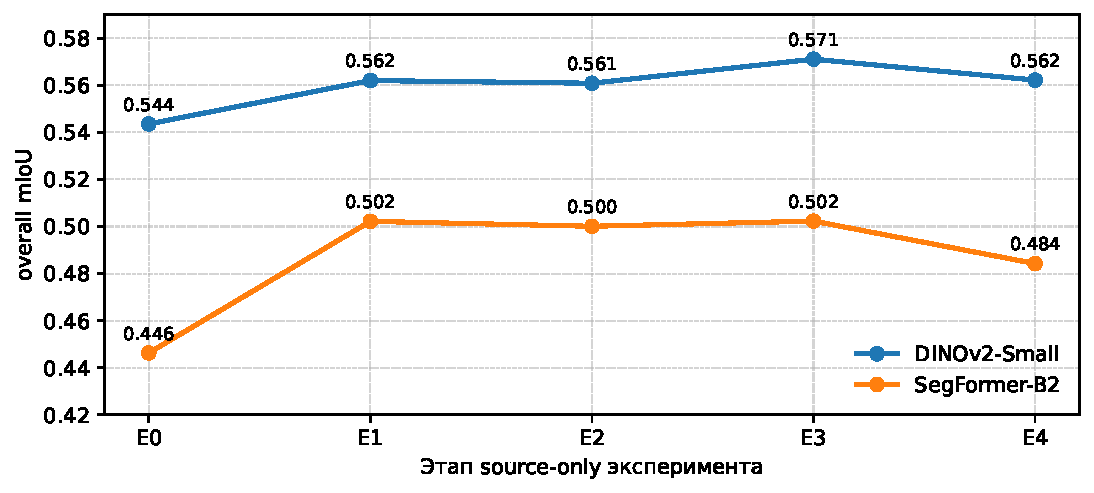
\includegraphics[width=0.82\textwidth]{source_only_dynamics.pdf}
    \caption{Динамика overall mIoU для DINOv2-Small и SegFormer-B2 в source-only экспериментах}
    \label{fig:source_only_dynamics}
\end{figure}

\subsection{Динамика E0--E4 для SegFormer-B2}

\subsubsection{Изменение метрик по этапам}

\begin{table}[H]
    \centering
    \caption{SegFormer-B2: source-only этапы E0--E4 на ACDC validation}
    \label{tab:segformer_e0_e4_metrics}
    \small
    \begin{tabular}{lrrrrrr}
        \toprule
        Этап & mIoU & PA & Fog & Night & Rain & Snow \\
        \midrule
        E0 & 0.4463 & 0.7685 & 0.5820 & 0.2461 & 0.4722 & 0.4553 \\
        E1 & 0.5022 & 0.8273 & 0.6330 & 0.2740 & 0.5232 & \textbf{0.5272} \\
        E2 & 0.5001 & 0.8249 & 0.6357 & 0.2881 & 0.5293 & 0.5158 \\
        E3 & \textbf{0.5023} & \textbf{0.8396} & \textbf{0.6426} & \textbf{0.2899} & \textbf{0.5328} & 0.5148 \\
        E4 & 0.4842 & 0.8277 & 0.6258 & 0.2761 & 0.4974 & 0.4859 \\
        \bottomrule
    \end{tabular}
\end{table}

У SegFormer-B2 основной прирост приходится на E1: mIoU растёт с $0.4463$ до $0.5022$. E2 и E3 изменяют результат на тысячные доли, а E4 заметно снижает качество. Формально лучший этап здесь тоже E3, но преимущество над E1 находится в пределах шума одного запуска.

\subsubsection{Сравнение с DINOv2-Small}

DINOv2-Small превосходит SegFormer-B2 на каждом этапе. Качественная картина изменений совпадает: E1 улучшает обе модели, E3 соответствует лучшему source-only результату, E4 снижает overall mIoU. Основное различие проявляется в трудных условиях. На ночи DINOv2-Small E3 удерживает $0.3823$, SegFormer-B2 E3 --- $0.2899$.

\subsection{Ошибки по условиям и классам}

\subsubsection{Night как самый сложный поддомен}

\textit{Night} остаётся самым сложным поддоменом во всех сериях. Даже у лучшего source-only DINOv2-Small E3 ночной mIoU равен $0.3823$, тогда как fog и snow находятся в районе $0.70$ и $0.60$. Слабое освещение ухудшает видимость границ объектов и снижает контраст между мелкими классами и фоном.

\subsubsection{Class-wise IoU и визуальные примеры}

\begin{table}[H]
    \centering
    \caption{Примеры class-wise IoU для трудных классов на лучших source-only этапах}
    \label{tab:hard_class_iou_source_only}
    \small
    \begin{tabular}{lrr}
        \toprule
        Класс & DINOv2-Small E3 & SegFormer-B2 E3 \\
        \midrule
        traffic light & 0.5184 & \textbf{0.5639} \\
        pole & 0.3888 & \textbf{0.4238} \\
        fence & \textbf{0.3691} & 0.2870 \\
        bicycle & \textbf{0.3314} & 0.2769 \\
        rider & \textbf{0.1689} & 0.1579 \\
        \bottomrule
    \end{tabular}
\end{table}

Низкие значения концентрируются на тонких и редких объектах. По отдельным классам преимущество не однозначно: SegFormer-B2 заметно лучше распознаёт \textit{traffic light} и \textit{pole}, но проигрывает на \textit{fence}, \textit{bicycle} и \textit{rider}. По всему ACDC и по большинству условий вперёд выходит DINOv2-Small E3.

На визуальных примерах (рис.~\ref{fig:dinov2_e3_examples}) виден типовой профиль ошибок: крупные области восстанавливаются уверенно, провалы концентрируются на границах, тонких структурах и мелких участниках движения. Эти примеры используются как дополнение к численным метрикам и помогают интерпретировать значения mIoU.

\newpage
\vspace*{-0.8cm}
\begin{figure}[H]
    \centering
    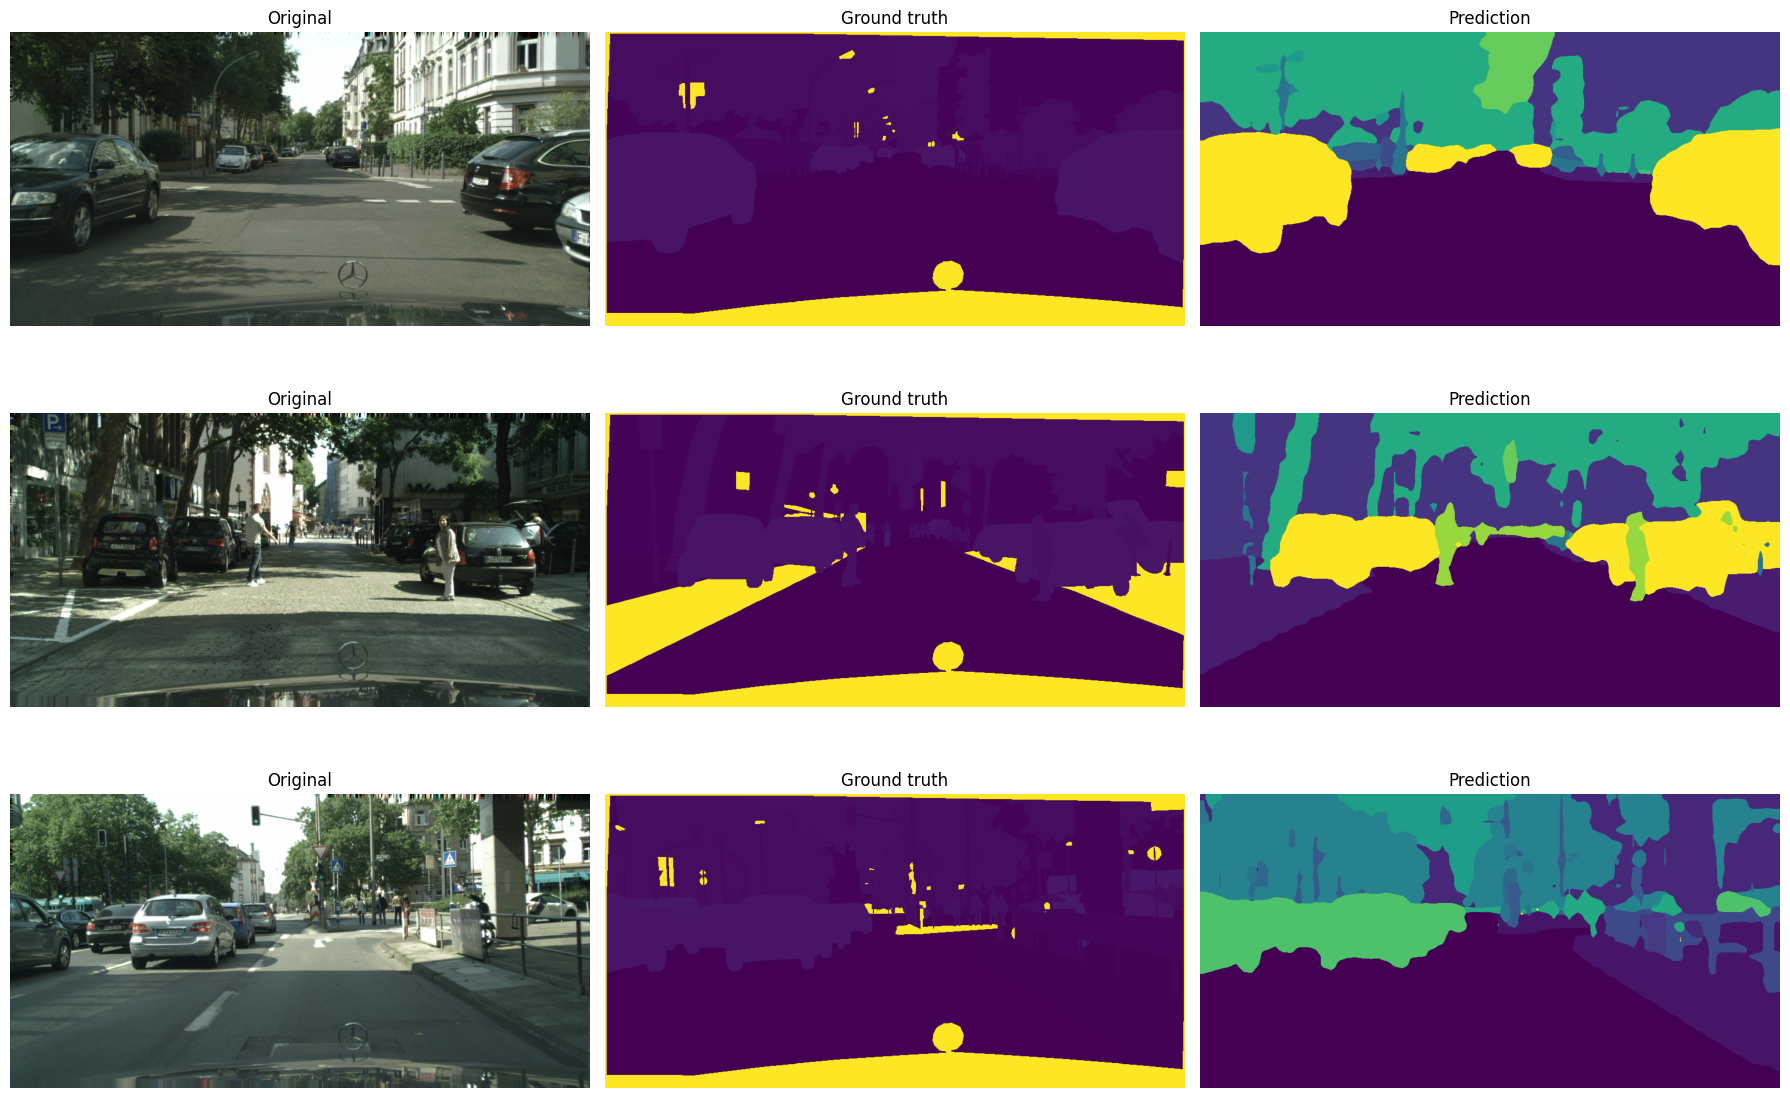
\includegraphics[width=0.68\textwidth]{../assets/dinov2_e3_segmentation_examples.png}
    \caption{Качественные примеры сегментации DINOv2-Small E3: изображение, ground truth и предсказание}
    \label{fig:dinov2_e3_examples}
\end{figure}

\newpage

\section{UDA-lite эксперименты на DINOv2-Small}

После source-only этапов отдельно проверяется постановка с дополнительной информацией о целевом домене: в обучение добавляются \textbf{неразмеченные изображения ACDC train}. Эта серия отделена от E0--E4, поскольку модель получает target-изображения, пусть и без ручной разметки.

\subsection{U1: self-training на pseudo-labels}

\subsubsection{Построение pseudo-labels для ACDC}

В U1 роль teacher играет лучшая source-only модель --- DINOv2-Small E3. Она проходит по ACDC train и для каждого пикселя сохраняет предсказанный класс только при уверенности $\max_k p^{(k)} \geq \tau$ с $\tau = 0.90$. Неуверенные пиксели маркируются ignore-меткой $255$ и выпадают из функции потерь. Обрабатывается 1600 изображений: по 400 на \textit{fog}, \textit{night}, \textit{rain}, \textit{snow}.

\begin{table}[H]
    \centering
    \caption{Статистика pseudo-labels для ACDC train в U1}
    \label{tab:u1_pseudo_label_stats}
    \small
    \begin{tabular}{lrrr}
        \toprule
        Условие & Изображений & Keep ratio & Confidence kept \\
        \midrule
        fog & 400 & 0.8297 & 0.9920 \\
        night & 400 & 0.6543 & 0.9871 \\
        rain & 400 & 0.8018 & 0.9906 \\
        snow & 400 & 0.7933 & 0.9897 \\
        \bottomrule
    \end{tabular}
\end{table}

Keep ratio просаживается на \textit{night} ($0.6543$): ночные кадры хуже всего размечаются source-only моделью, поэтому teacher чаще отбрасывает неуверенные пиксели. На остальных условиях keep ratio держится в районе $0.80$, средняя уверенность сохранённых пикселей --- около $0.99$ (рис.~\ref{fig:pseudo_label_keep_ratio}).

\begin{figure}[H]
    \centering
    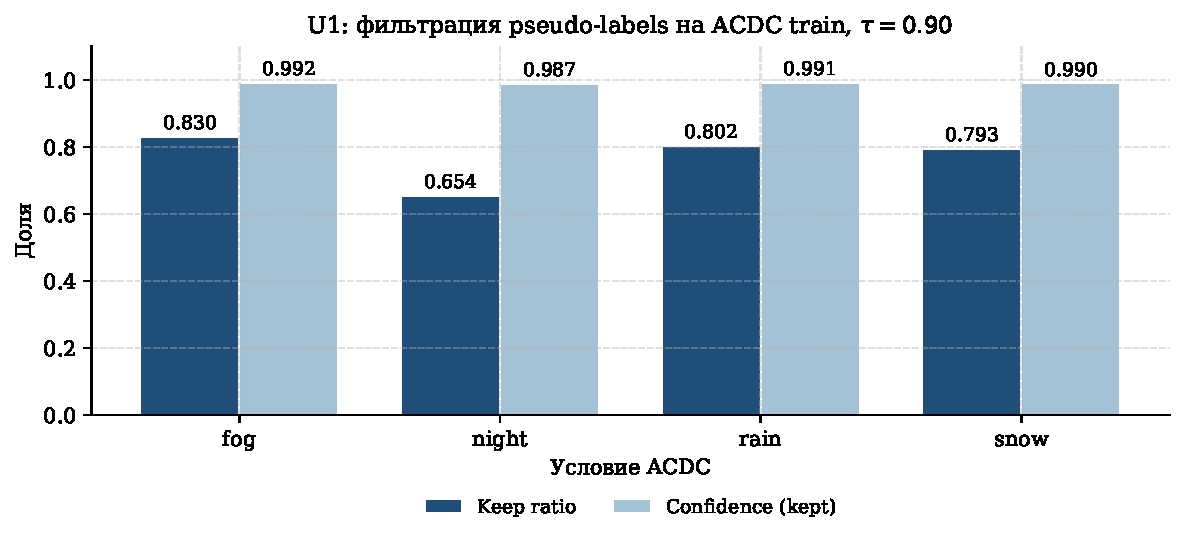
\includegraphics[width=0.78\textwidth]{pseudo_label_keep_ratio.pdf}
    \caption{U1: доля сохранённых пикселей и средняя уверенность кадров ACDC train при $\tau=0.90$}
    \label{fig:pseudo_label_keep_ratio}
\end{figure}

\subsubsection{Дообучение и результат U1}

Дообучение проводится на смеси размеченного Cityscapes и ACDC train с pseudo-labels. В качестве начальных весов используется checkpoint DINOv2-Small E3; U1 продолжает обучение модели с наилучшим source-only результатом и добавляет target-данные без ручной разметки.

На ACDC validation overall mIoU поднимается с $0.5711$ до $\mathbf{0.5828}$. Наибольший прирост приходится на \textit{rain}: $0.5542 \to 0.5898$ ($+0.036$). Confidence-фильтр улучшает результат без архитектурных изменений.

\subsection{U2: EMA teacher и ClassMix}

\subsubsection{EMA teacher для online pseudo-labeling}

U2 заменяет фиксированный teacher на скользящее среднее. Веса EMA-teacher обновляются как $\theta_{t} = \alpha\,\theta_{t-1} + (1-\alpha)\,\theta_{\text{student}}$ с $\alpha = 0.999$. Pseudo-labels формируются прямо в обучающем цикле, а порог уверенности постепенно снижается с $0.968$ до $0.90$.

EMA-teacher снижает зависимость от одного фиксированного teacher-снимка. На ранних итерациях порог строже отбирает target-пиксели, а к концу обучения допускает больше target-сигнала, когда student уже стабилизировался.

\subsubsection{ClassMix и результат U2}

К EMA-teacher добавляется ClassMix: на одном изображении смешиваются классовые регионы из source-кадра и target-кадра. Такой прием расширяет распределение комбинаций объект--фон, по которым student получает обучающий сигнал. В реализации ClassMix включается с вероятностью $0.5$, обучение стартует от U1-checkpoint.

Итоговый overall mIoU равен $\mathbf{0.5957}$, что является максимальным значением среди всех экспериментов: $+0.0129$ относительно U1 и $+0.0246$ относительно лучшего source-only этапа E3.

\subsection{Сравнение E3, U1 и U2}

\subsubsection{Итоговые метрики}

\begin{table}[H]
    \centering
    \caption{Сравнение лучшего source-only этапа и UDA-lite экспериментов}
    \label{tab:e3_u1_u2_comparison}
    \small
    \begin{tabular}{lrrrrrr}
        \toprule
        Этап & mIoU & PA & Fog & Night & Rain & Snow \\
        \midrule
        E3 & 0.5711 & 0.8826 & 0.6977 & 0.3823 & 0.5542 & 0.6004 \\
        U1 & 0.5828 & 0.8867 & 0.7001 & 0.3887 & 0.5898 & 0.5977 \\
        U2 & \textbf{0.5957} & \textbf{0.8923} & \textbf{0.7055} & \textbf{0.3980} & \textbf{0.6058} & \textbf{0.6087} \\
        \bottomrule
    \end{tabular}
\end{table}

\begin{figure}[H]
    \centering
    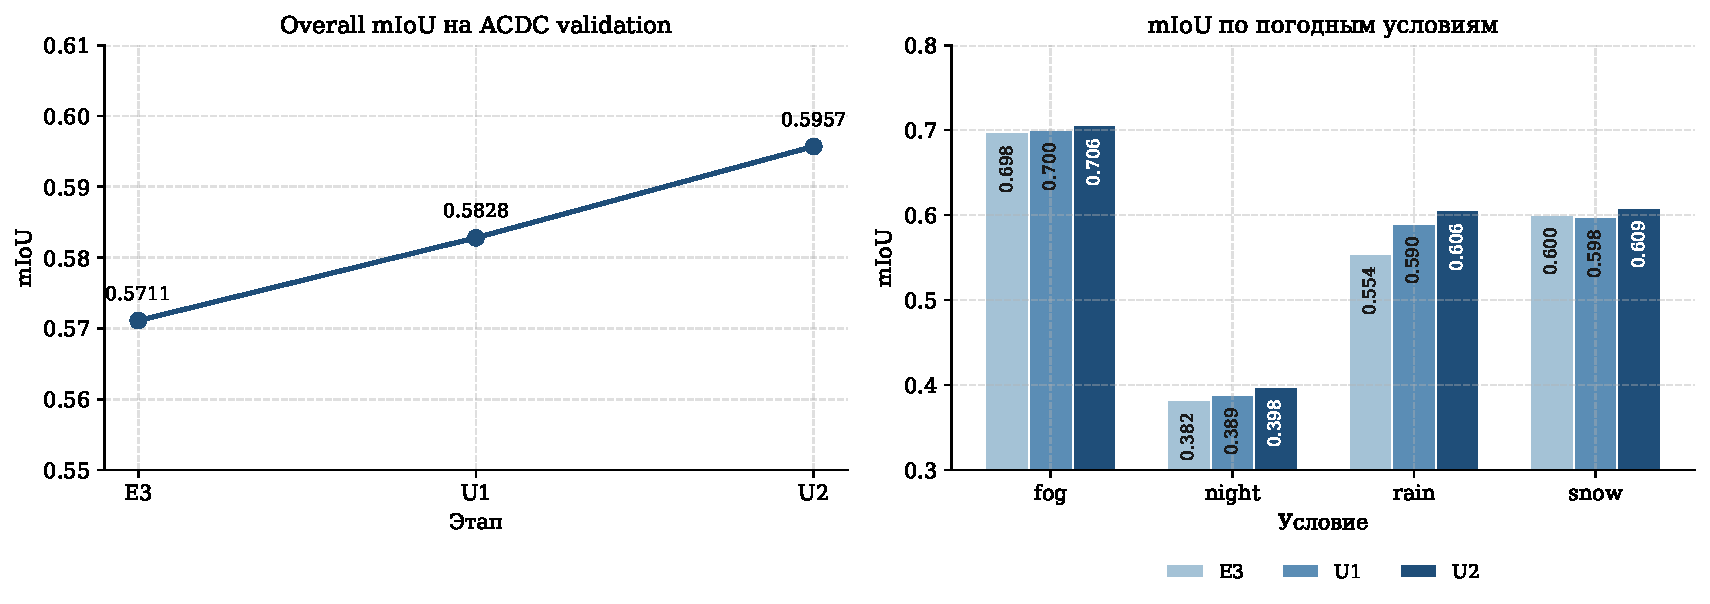
\includegraphics[width=\textwidth]{uda_lite_progression.pdf}
    \caption{DINOv2-Small: переход E3 $\to$ U1 $\to$ U2 на ACDC validation. Слева --- overall mIoU, справа --- per-condition разбиение}
    \label{fig:uda_lite_progression}
\end{figure}

В последовательности E3 $\to$ U1 $\to$ U2 качество монотонно растет (рис.~\ref{fig:uda_lite_progression}). U2 показывает наибольшее значение overall mIoU и лучший результат по каждому из четырёх поддоменов.

\subsubsection{Изменение качества по погодным условиям}

Самый крупный прирост относительно E3 фиксируется на \textit{rain}: $+0.0516$ mIoU в U2. На \textit{night} улучшение меньше ($0.3823 \to 0.3980$), но сохраняется на обоих UDA-lite этапах. Ночные сцены остаются наиболее сложными: fog и snow находятся выше $0.60$, а night остаётся ниже $0.40$.

\begin{figure}[H]
    \centering
    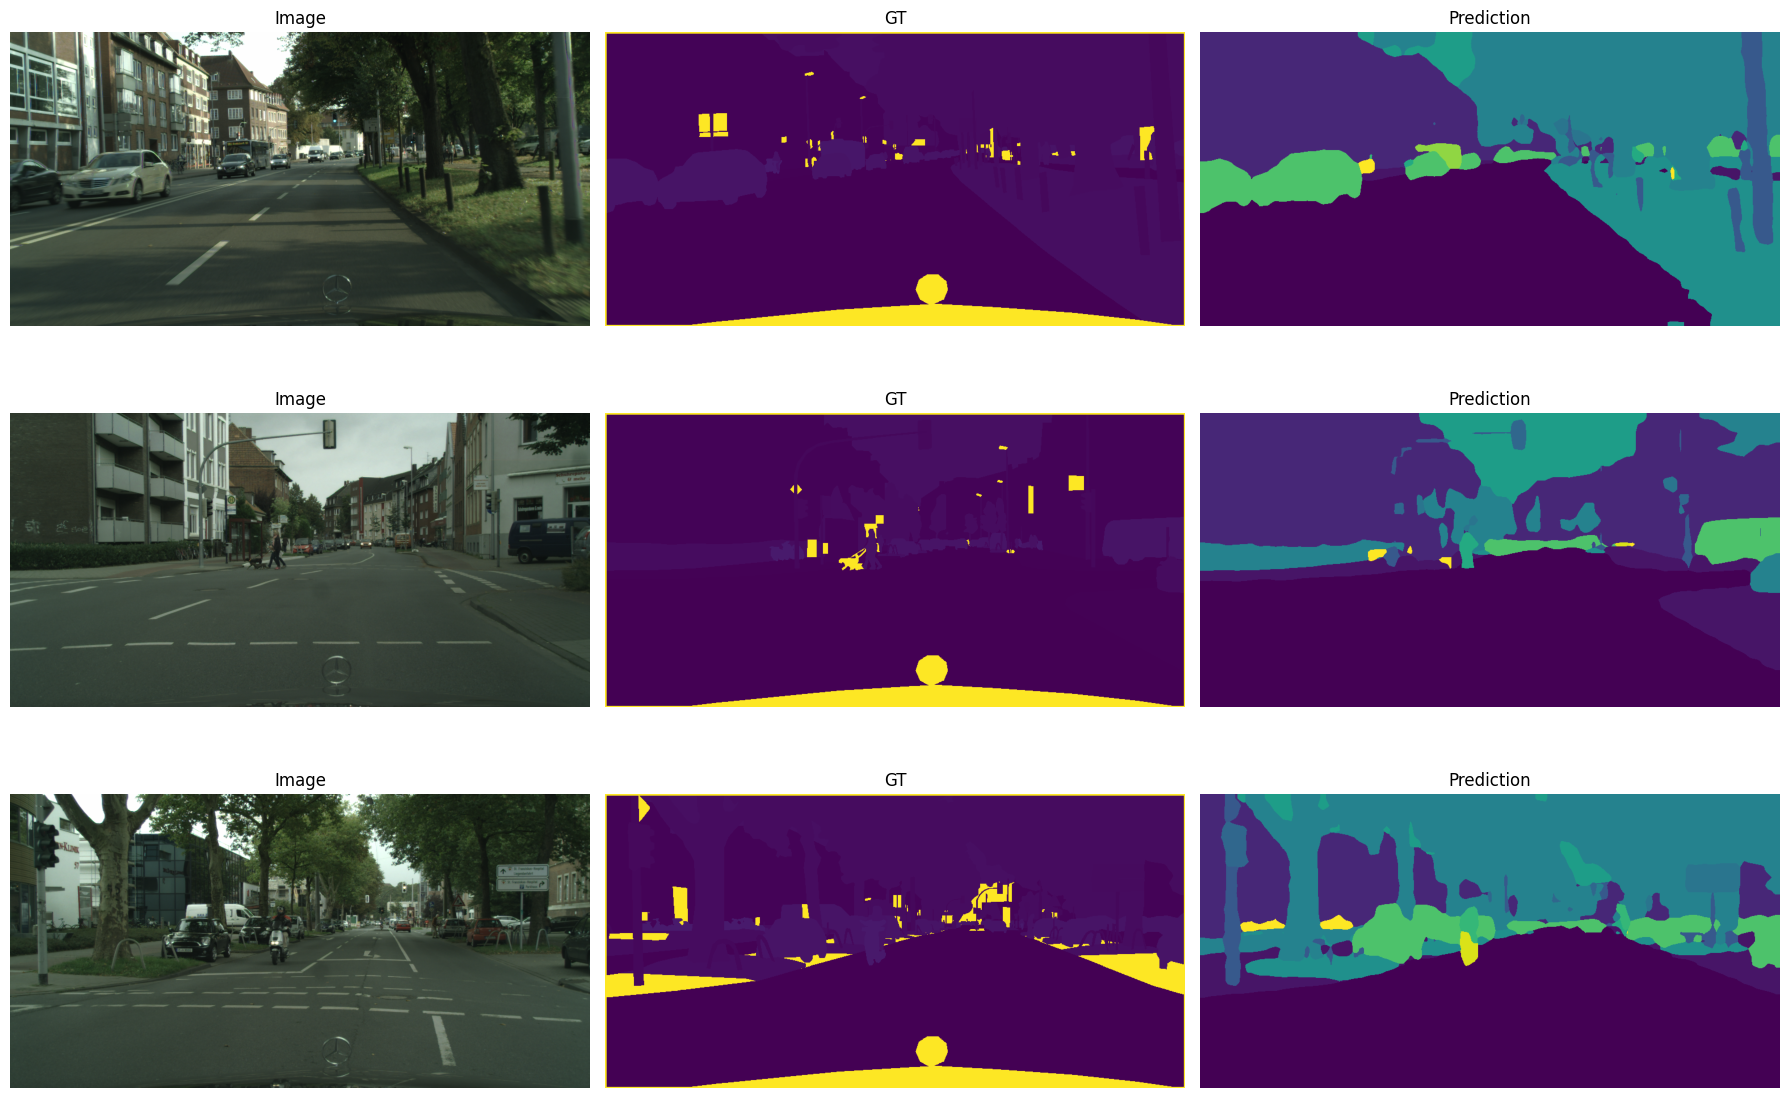
\includegraphics[width=0.68\textwidth]{../assets/dinov2_u1_segmentation_examples.png}
    \caption{Качественные примеры сегментации DINOv2-Small U1: изображение, ground truth и предсказание}
    \label{fig:dinov2_u1_examples}
\end{figure}

Полученные результаты задают два сценария использования. При отсутствии target-данных на этапе обучения предпочтительным вариантом остается DINOv2-Small E3. При наличии неразмеченных изображений ACDC train более высокое качество показывает DINOv2-Small U2.

\newpage

\section{Обсуждение результатов и ограничений}

\subsection{Основные экспериментальные выводы}

\subsubsection{Архитектура как главный фактор качества}

Наибольшее влияние на качество оказывает выбор архитектуры. В E0 DINOv2-Small достигает $0.5436$ mIoU, SegFormer-B2 --- $0.4463$, InternImage-Tiny --- $0.3899$, DeepLabV3+ --- $0.3015$. Разрыв между крайними значениями превышает $0.24$ overall mIoU, что больше любого прироста от source-only модификаций. Следовательно, аугментации не компенсируют ограничения слабого backbone.

\subsubsection{Эффект source-only модификаций}

Source-only приёмы обеспечивают умеренное, но воспроизводимое улучшение. Лучший этап E3 поднимает DINOv2-Small с $0.5436$ до $0.5711$ ($+0.028$) и SegFormer-B2 с $0.4463$ до $0.5023$ ($+0.056$). E4 не подтверждает пользу consistency-регуляризации в этой реализации: на обеих моделях overall mIoU после него падает по сравнению с E3.

В этой серии фотометрические аугментации и frequency-style преобразования повышают устойчивость переноса. Их эффект ограничен отсутствием данных из target-распределения.

\subsubsection{Вклад UDA-lite}

Максимальное итоговое качество достигается в UDA-lite. U1 показывает, что offline pseudo-labeling улучшает DINOv2-Small E3 ($0.5711 \to 0.5828$). U2 с EMA-teacher и ClassMix добавляет ещё $+0.013$ и достигает $0.5957$ mIoU. Неразмеченные изображения ACDC содержат информацию о target-распределении, недоступную source-only приемам.

Результаты UDA-lite и E0--E4 следует интерпретировать раздельно, поскольку эти серии различаются постановкой задачи и уровнем доступа к данным.

\subsection{Ограничения исследования}

\subsubsection{Ограниченное число повторных запусков}

Ключевые конфигурации запускались несколько раз, но число повторов осталось ограниченным. Доверительных интервалов нет, поэтому различия порядка нескольких тысячных mIoU следует считать шумом обучения --- особенно для близких пар вроде SegFormer-B2 E1 и E3. В выводах учитываются только эффекты, заметно превышающие такой разброс: преимущество DINOv2-Small, прирост на E3 и переход к UDA-lite.

\subsubsection{ACDC validation и границы сопоставимости}

Все числа получены на ACDC validation. Такой протокол подходит для сопоставления этапов внутри работы, но публичные лидерборды используют закрытое test-разбиение и другие протоколы обучения, поэтому численного сравнения с ними результаты работы не подразумевают.

UDA-lite реализован только для DINOv2-Small. Перенос U1 и U2 на SegFormer-B2 требует отдельной проверки.

\subsection{Рекомендации по использованию результатов}

\subsubsection{Выбор режима обучения}

Если target-домен недоступен на этапе обучения, среди проведённых экспериментов предпочтителен DINOv2-Small E3. Он показывает лучший source-only результат и не использует ACDC при обучении. При наличии неразмеченных изображений target-домена наибольшее качество показывает DINOv2-Small U2: он лидирует по overall mIoU и по каждому из четырёх условий.

SegFormer-B2 E3 можно рассматривать как более простую альтернативу, однако по качеству переноса он заметно уступает DINOv2-Small.

\subsubsection{Направления дальнейшей проверки}

Дальнейшая проверка должна включать повторение ключевых запусков с несколькими seed, оценку на независимом test-разбиении и отдельный анализ ночных сцен. \textit{Night} остаётся главным слабым местом: даже U2 поднимает его только до $0.3980$ mIoU.

Также требуется проверить UDA-lite для SegFormer-B2, чтобы отделить вклад метода адаптации от вклада foundation-признаков DINOv2.

\newpage

\section*{Заключение}
\addcontentsline{toc}{section}{Заключение}

В работе изучен перенос моделей семантической сегментации дорожных сцен из Cityscapes в ACDC: из дневной городской съёмки в сцены с туманом, ночью, дождём и снегом. Цель исследования состояла в сравнении архитектур и приёмов обучения при ограниченном доступе к target-домену.

Наибольшее качество среди baseline-архитектур показала DINOv2-Small. Уже в E0 она достигает $0.5436$ mIoU на ACDC validation, опережая SegFormer-B2, InternImage-Tiny и DeepLabV3+. Дальнейшие эксперименты были сосредоточены на DINOv2 и SegFormer-B2 как контрольной transformer-based архитектуре.

Из source-only модификаций лучшим оказался этап E3 с частотными преобразованиями: DINOv2-Small поднимается до $0.5711$ mIoU, SegFormer-B2 --- до $0.5023$. E4 устойчивого прироста не дал и на обеих моделях откатил overall mIoU ниже E3.

Серия UDA-lite показала, что неразмеченные ACDC-изображения содержат полезную информацию о target-распределении. Offline self-training на pseudo-labels (U1) поднимает DINOv2-Small E3 до $0.5828$ mIoU; EMA-teacher с ClassMix (U2) достигает лучшего итогового значения --- $\mathbf{0.5957}$ mIoU. Значение остаётся ниже верхних позиций лидерборда HyperAI, но подтверждает совместный вклад foundation-признаков DINOv2 и target-данных без ручной разметки.

\textit{Night} остаётся самым проблемным поддоменом во всех сериях. Даже U2 удерживает на нём $0.3980$ mIoU, тогда как fog, rain и snow находятся в районе $0.6$--$0.7$. Поэтому дальнейшая работа должна включать более сильные аугментации освещения, отдельный анализ редких классов и повторные запуски с несколькими seed для оценки дисперсии.

\newpage
\printbibliography[heading=bibintoc, title={Список использованной литературы}]

\newpage

\section*{Приложение 1. Сводные таблицы метрик и class-wise IoU}
\addcontentsline{toc}{section}{Приложение 1. Сводные таблицы метрик и class-wise IoU}

В основной части приведены только таблицы, нужные для интерпретации результатов. Полная агрегация метрик собрана в ноутбуке \texttt{notebooks/eval/ACDC\_Eval\_Metrics\_Comparison.ipynb}, где доступны:
\begin{itemize}
    \item overall mIoU и Pixel Accuracy для E0--E4, U1 и U2;
    \item per-condition mIoU для \textit{fog}, \textit{night}, \textit{rain}, \textit{snow};
    \item приивросты между соседними этапами;
    \item class-wise IoU из отдельных evaluation-ноутбуков.
\end{itemize}

\begin{table}[H]
    \centering
    \caption{Краткая сводка ключевых итоговых результатов}
    \label{tab:appendix_key_results}
    \small
    \begin{tabular}{lll}
        \toprule
        Сценарий & Лучшая модель / этап & Overall mIoU \\
        \midrule
        Baseline E0 & DINOv2-Small E0 & 0.5436 \\
        Source-only & DINOv2-Small E3 & 0.5711 \\
        UDA-lite offline & DINOv2-Small U1 & 0.5828 \\
        UDA-lite online & DINOv2-Small U2 & \textbf{0.5957} \\
        Лучший SegFormer & SegFormer-B2 E3 & 0.5023 \\
        \bottomrule
    \end{tabular}
\end{table}

\newpage

\section*{Приложение 2. Визуализации предсказаний и параметры запусков}
\addcontentsline{toc}{section}{Приложение 2. Визуализации предсказаний и параметры запусков}

Качественные примеры сегментации находятся в каталоге \texttt{assets/}. В тексте использованы \texttt{dinov2\_e3\_segmentation\_examples.png} и \texttt{dinov2\_u1\_segmentation\_examples.png}. Эти визуализации показывают, где модель корректно выделяет крупные области, а где теряет тонкие объекты и границы.

Параметры запусков зафиксированы внутри train- и eval-ноутбуков. Основные точки входа:
\begin{itemize}
    \item \texttt{notebooks/train/cityscapes/e3/} --- лучший source-only этап;
    \item \texttt{notebooks/pseudo/acdc/u1/} --- генерация pseudo-labels для ACDC train;
    \item \texttt{notebooks/train/cityscapes\_acdc/u1/} --- offline self-training;
    \item \texttt{notebooks/train/cityscapes\_acdc/u2/} --- EMA teacher и ClassMix;
    \item \texttt{notebooks/eval/acdc/} --- оценка на ACDC validation.
\end{itemize}

Для воспроизводимости вместе с checkpoint сохраняется и ноутбук запуска: в нём зафиксированы размер входа, batch size, learning rate, число эпох, состав аугментаций и путь к весам.
\end{document}